%\textbf{\large 11. FIR filters}
%\\
%
%\begin{align}
%	H(\omega) &= \sum_{n=-\infty}^\infty h_n e^{-i \omega n} \\
%	&= h_{-1} e^{i \omega} + h_0 e^{0} + h_1 e^{-i \omega} \\
%	&= h_0 + h_1 \left( e^{i \omega} + e^{-i \omega} \right) & & \text{with}\ h_{-1} = h_1 \\
%	&= h_0 + 2 h_1 \cos(\omega) \\
%\end{align}
%
%
%\textbf{a)} $\{h_{-1}, h_0, h_1\} = \left\{\frac{1}{3}, \frac{1}{3}, \frac{1}{3}\right\}$
%
%\begin{equation*}
%	H(\omega) = \frac{1}{3} + \frac{2}{3} \cos(\omega)
%\end{equation*}
%
%\textbf{b)} $\{h_{-1}, h_0, h_1\} = \left\{\frac{1}{4}, \frac{1}{2}, \frac{1}{4}\right\}$
%
%\begin{equation*}
%	H(\omega) = \frac{1}{2} + \frac{1}{2} \cos(\omega)
%\end{equation*}
%
%\textbf{c)} $\{h_{-1}, h_0, h_1\} = \left\{-\frac{1}{4}, \frac{1}{2}, -\frac{1}{4}\right\}$
%
%\begin{equation*}
%	H(\omega) = \frac{1}{2} - \frac{1}{2} \cos(\omega)
%\end{equation*}
%
%\vspace{1cm}
%Since all filters are symmetric around the orgin, the phase is zero.
%
%\begin{figure}[h]
%	\centering
%	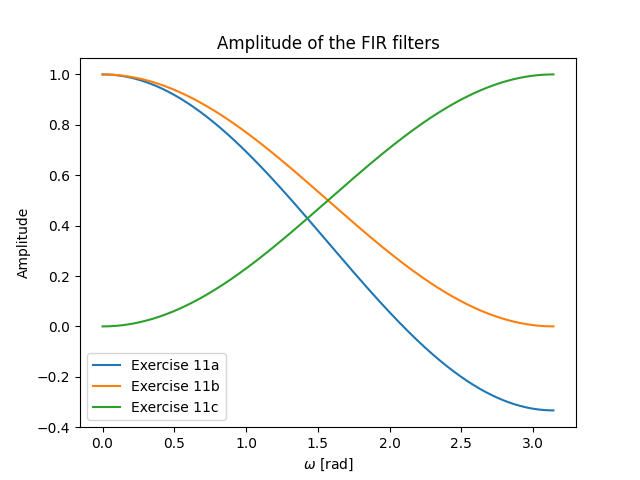
\includegraphics[width=12cm]{img/ex_11.png}
%	\captionsetup{width=10cm}
%	\caption{Amplitudes for the given FIR filters.}
%\end{figure}


\textbf{\large 12. Multipying frequency responses}
\\

\textbf{a) Amplitude Plot}\\

Given that:

\begin{align}
	H_b(\omega) &= \frac{1}{4} + \frac{1}{2} \cos(\omega) \\
	H_c(\omega) &= \frac{1}{4} - \frac{1}{2} \cos(\omega) \\
	\cos^2(x) &= \frac{1+\cos(x)}{2}
\end{align}

Follows:

\begin{align*}
	H_{bc}(\omega) &= H_b(\omega) H_c(\omega) \\
	&= \frac{1}{4} + \frac{1}{2} \cos(\omega) - \frac{1}{2} \cos(\omega) - \frac{1}{4} \cos^2(\omega)\\
	&= \frac{1}{4} - \frac{1}{4} \cos^2(\omega) \\
	&= \frac{1}{4} - \frac{1}{4} \frac{1+\cos(2\omega)}{2} \\
	&= \frac{1}{4} - \frac{1}{8} - \frac{1}{8}\cos(2\omega) \\
	&= \frac{1}{8} - \frac{1}{8} \cos(2\omega) \\
	&= \frac{1}{8} \left(1 - \cos(2\omega)\right)
\end{align*}

\begin{figure}[h]
	\centering
	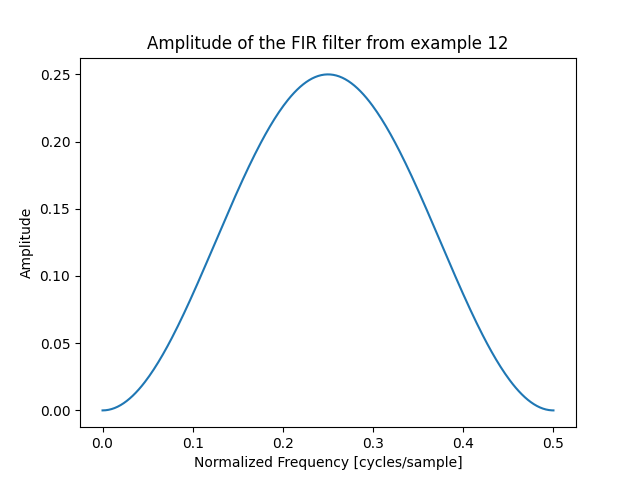
\includegraphics[width=7cm]{img/ex_12.png}
	\captionsetup{width=5cm}
	\caption{Amplitude for the given FIR filters.}
\end{figure}

\newpage

\textbf{b) Time Domain Coefficiants} \\

Given that:

\begin{align}
	H_{bc}(\omega) &= \frac{1}{8} - \frac{1}{8} \cos(2\omega) \\
	\cos(x) &= \frac{e^x + e^{-x}}{2}
\end{align}

Follows:

\begin{align*}
	\frac{1}{8} - \frac{1}{8} \cos(2\omega) &= \frac{1}{8} - \frac{1}{8} \frac{e^{2i\omega} + e^{-2i\omega}}{2} \\ 
	&= -\frac{1}{16} e^{2i\omega} + \frac{1}{8} e^{0i\omega} - \frac{1}{16} e^{-2i\omega} \\
	&\Rightarrow \left\{ -\frac{1}{16},\ 0,\ \frac{1}{8},\ 0,\ -\frac{1}{16} \right\}
\end{align*}

\textbf{\large 13. IRR filter}
\\

Given that:

\begin{align}
	\{a_{-1},\ a_0,\ a_1\} &= \left\{-\frac{1}{2},\ 1,\ 0\right\} \\
	\{b_{-1},\ b_0,\ b_1\} &= \left\{\frac{1}{8},\ \frac{1}{4},\ \frac{1}{8}\right\}
\end{align}
Follows:

\begin{align*}
	H(\omega) &= \frac{Y(\omega)}{X(\omega)}\\
	&= \frac{\frac{1}{8} e^{i\omega} + \frac{1}{4} + \frac{1}{8} e^{-i\omega}}{-\frac{1}{2} e^{i\omega} + 1}\\
	&= \frac{\frac{1}{4} (1 + cos(\omega))}{1 - \frac{1}{2} e^{i\omega}}
	&= \frac{1 + cos(\omega)}{4 - 2 e^{i\omega}}
\end{align*}

\begin{figure}[h]
	\centering
	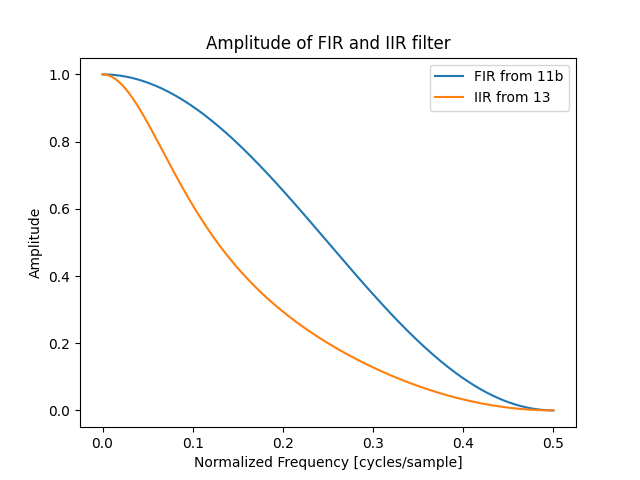
\includegraphics[width=8cm]{img/ex_13.png}
	\captionsetup{width=6cm}
	\caption{Amplitude comparison for the filters from example 11a and 13.}
\end{figure}
